\subsection{Characterizing individual features}

As a first step of actual data exploration, we are now going to look at which information we can get from a single data feature. In terms of tabular data: we're going to focus on a single column.

What kind of data we can derive from the feature, depends of course on the data type. Generally deriving features from other ones is of course done best when dealing with structured data. Here, we have two types from which we can derive different properties.

From \textbf{continuous features}, we can derive\sidenote{Properties from investigating individual \textbf{continuous} feature}\renewcommand{\arraystretch}{1.5}

\begin{tabular}{@{}>{\raggedleft}m{0.2\textwidth} @{}>{\color{black}\centering:}m{0.025\textwidth} @{}>{\color{black}}m{0.775\textwidth}}
  count && Number of instances having this feature \\
  \% miss && Percentage of missing information {\color{gray}\footnotesize(how many instances don't have this feature)} \\
  card && Number of unique values (cardinality) \\
  min && Minimal value over all instances \\
  1\textsuperscript{st} qrt && 25\textsuperscript{th} percentile {\color{gray}\footnotesize(largest value of the quarter of instances having the lowest values)} \\
  mean && Average value over all instances \\
  median && Middle value of all instances \\
  3\textsuperscript{rd} qrt && 75\textsuperscript{th} percentile {\color{gray}\footnotesize(smallest value of the quarter of instances having the highest values)} \\
  max && Maximal value over all instances \\
  std. dev && Standard deviation over all instances
\end{tabular}


From \textbf{categorical features}, we can derive\sidenote{Properties from investigating individual \textbf{categorical} feature}\footnote{obvious: $\min$, $\max$, {\color{mathblue}mean}, etc. can't be computed}

\begin{tabular}{@{}>{\raggedleft}m{0.2\textwidth} @{}>{\color{black}\centering:}m{0.025\textwidth} @{}>{\color{black}}m{0.775\textwidth}}
  count && Number of instances having this feature \\
  \% miss && Percentage of missing information {\color{gray}\footnotesize(how many instances don't have this feature)} \\
  card && Number of unique values (cardinality) \\
  mode && Most common value \\
  mode frequ && Frequency of the mode \\
  mode \% && Percentage of the mode \\
  2\textsuperscript{nd}\,mode && Second most common value \\
  2\textsuperscript{nd}\,mode frequ && Frequency for the second mode \\
  2\textsuperscript{nd}\,mode \% && Percentage of the second mode
\end{tabular}

To get a better idea of how to get these properties for all of the features, we will look at an example. Consider a table containing information about insurance claims fraud. The dataset contains 500 instances (claims) and a bunch of different features such as type, claim amount, etc. Now first, determine the data type of each feature, and then create one table for the numerical and one for the categorical features and fill it with the according information. The original data and the resulting feature-describing tables can be found in \ref{fig:2_single_feature_example}.

\begin{figure}[H]
  \centering
  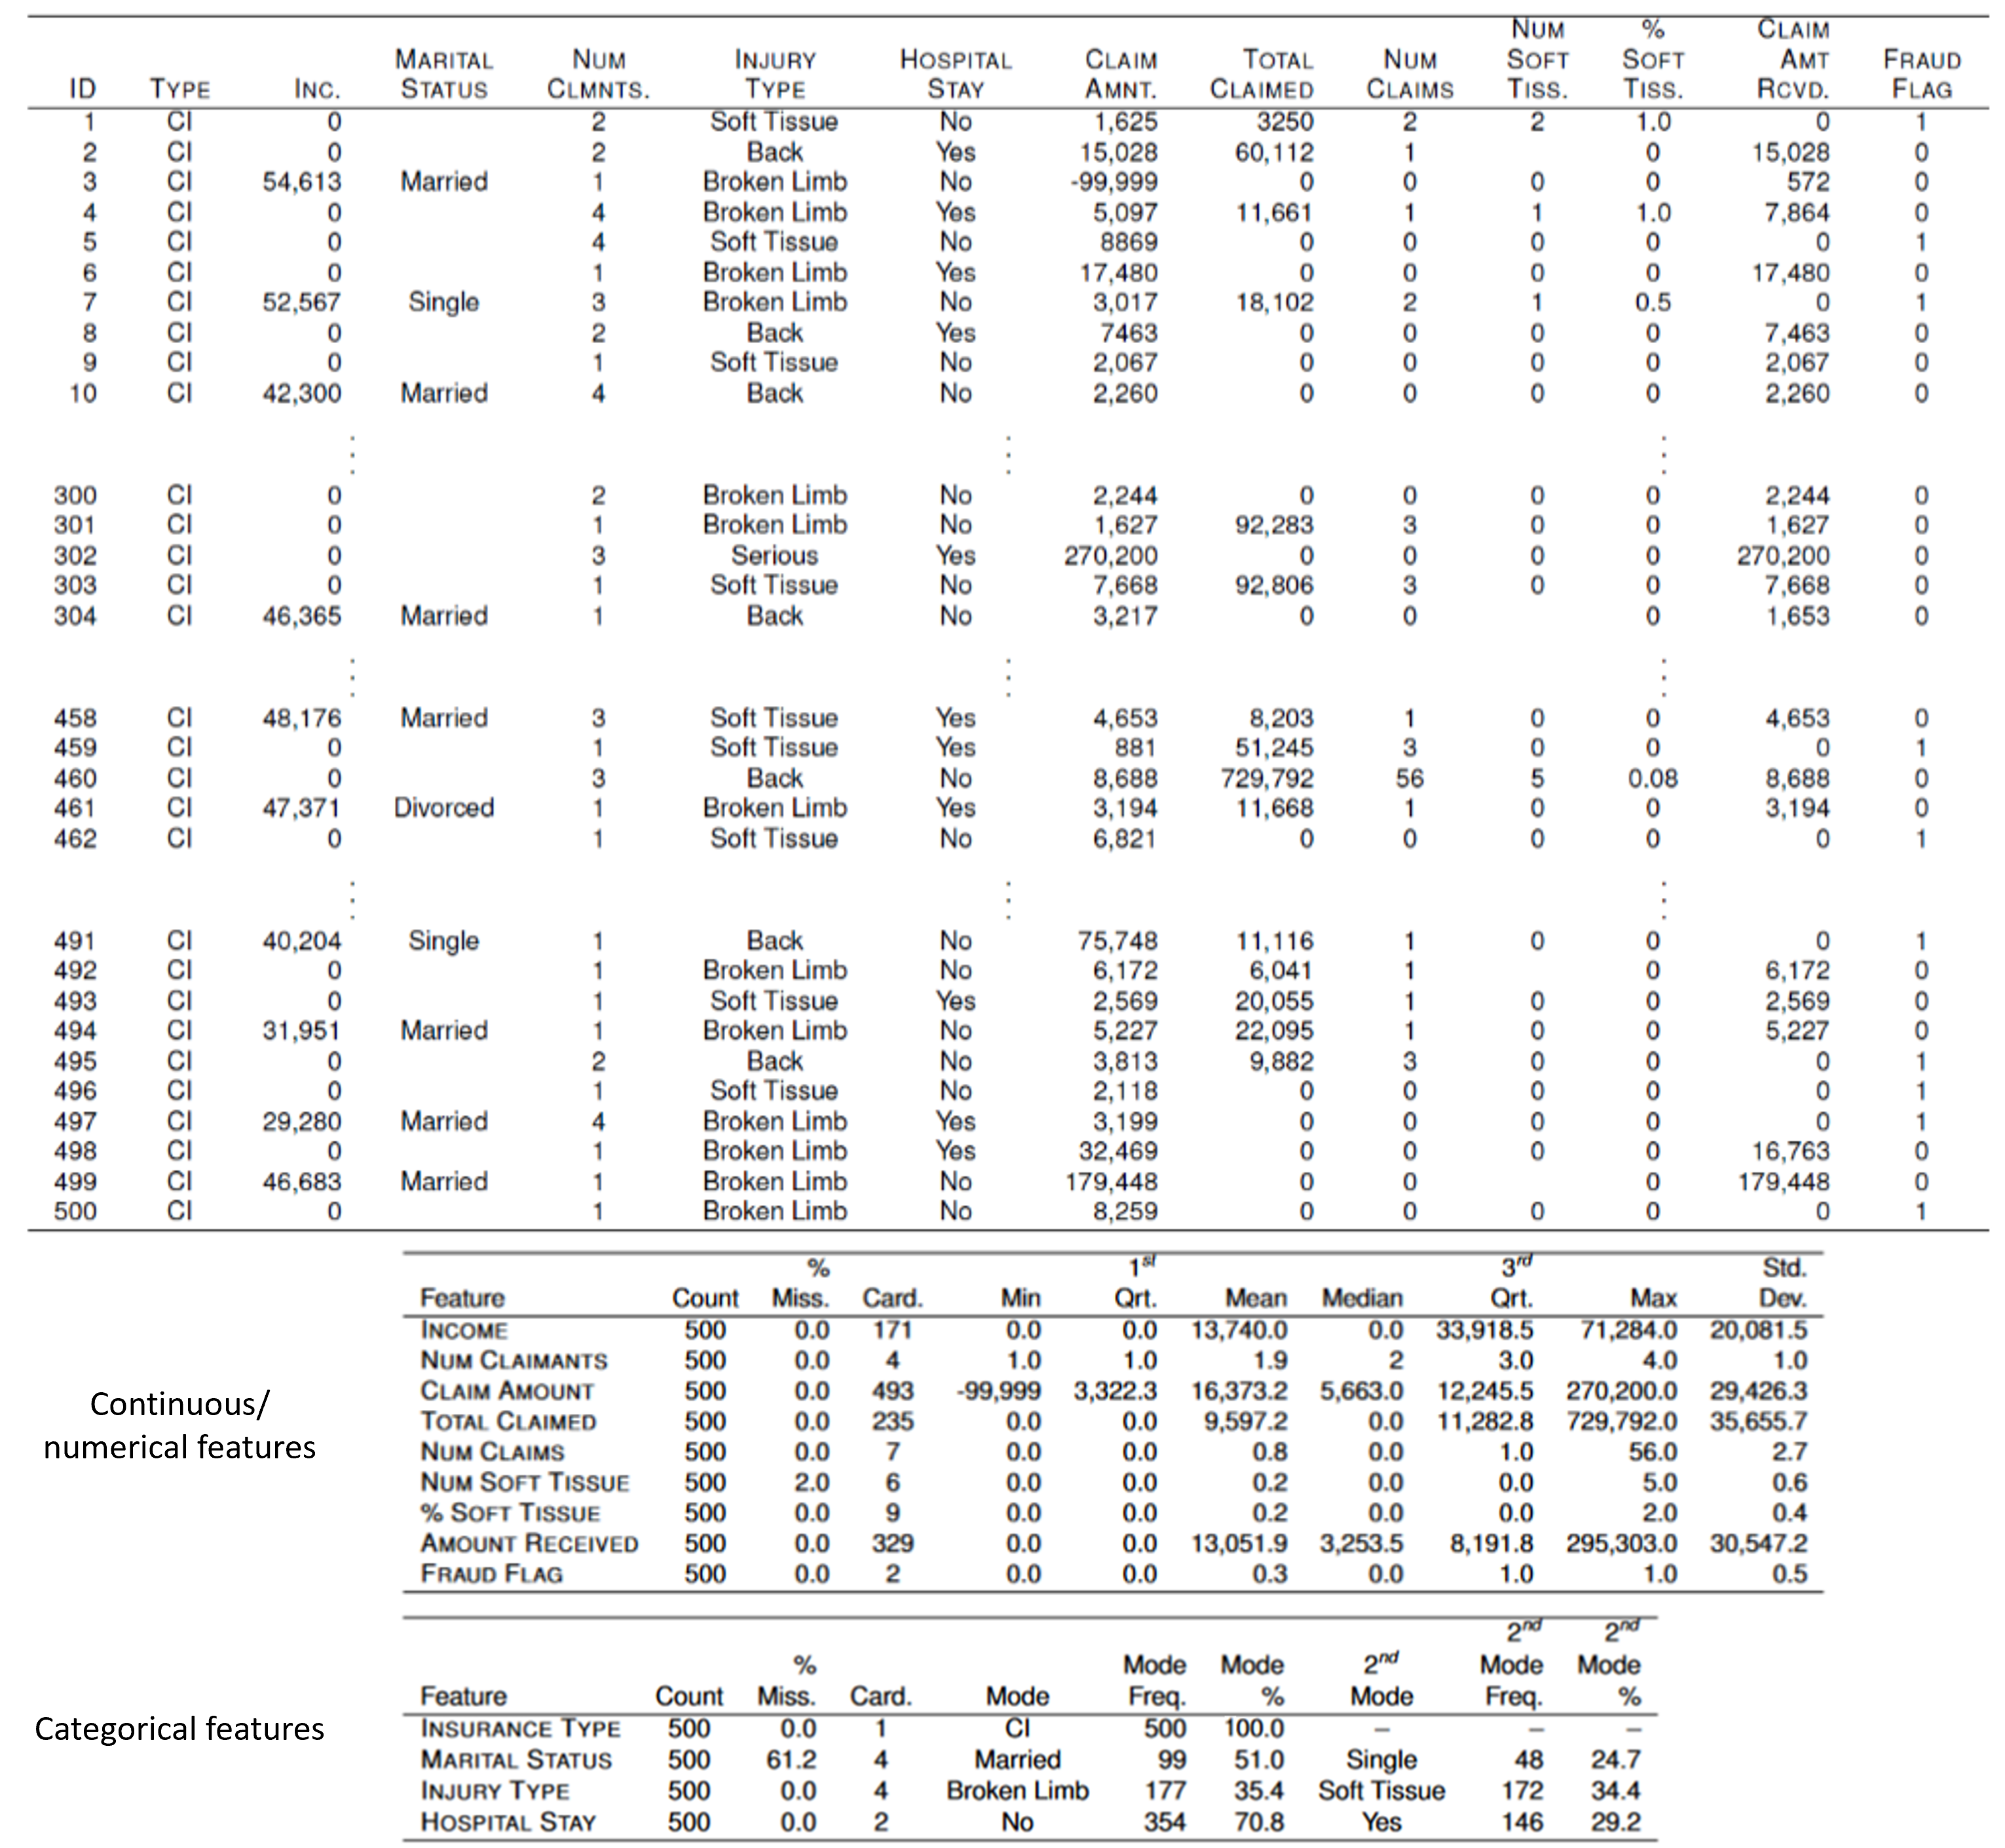
\includegraphics[width=\textwidth]{assets/visualization_and_extraction/example_single_featue.png}
  \caption{Example for single feature investigation (insurance claim fraud)}
  \label{fig:2_single_feature_example}
\end{figure}

To investigate the raw data further, let's visualize it. More specifically, we're going to visualize the distributions of the different features.
\begin{itemize}
  \item For finite amounts of possible feature classes, simply visualize the distribution as a bar diagram with the different classes as entries on the x-axis. The y-axis can either be the frequency or a percentage.
  \item For continuous features with continuous variables/infinitely many possible feature values, group items (\textbf{binning}\sidenote{Binning}) and then visualize the resulting histogram.
\end{itemize}


